Seit der Entdeckung der kosmischen Höhenstrahlung
1912 von Victor Hess feiert die Astroteilchenphysik bahnbrechende Errungenschaften.
Die Entdeckung der kosmischen Hintergrundstrahlung gilt als Beleg des
expandierenden Universums und wirft dennoch weitere Fragen zum frühen Universum auf.
Durch kosmische Botenteilchen ist das Erforschen von elementaren Bausteine und
Beschleunigungsprozessen möglich.
Anhand von kosmischen Botenteilchen können Informationen über Supernovae,
Aktive Galaxienkerne und weitere kosmische Phänomene, wie zum Beispiel
Neutronensterne und Gamma Ray Bursts, gewonnen werden.

\section*{MAGIC}%
\label{sec:magic}

\begin{wrapfigure}[13]{O}{0.45\textwidth}
		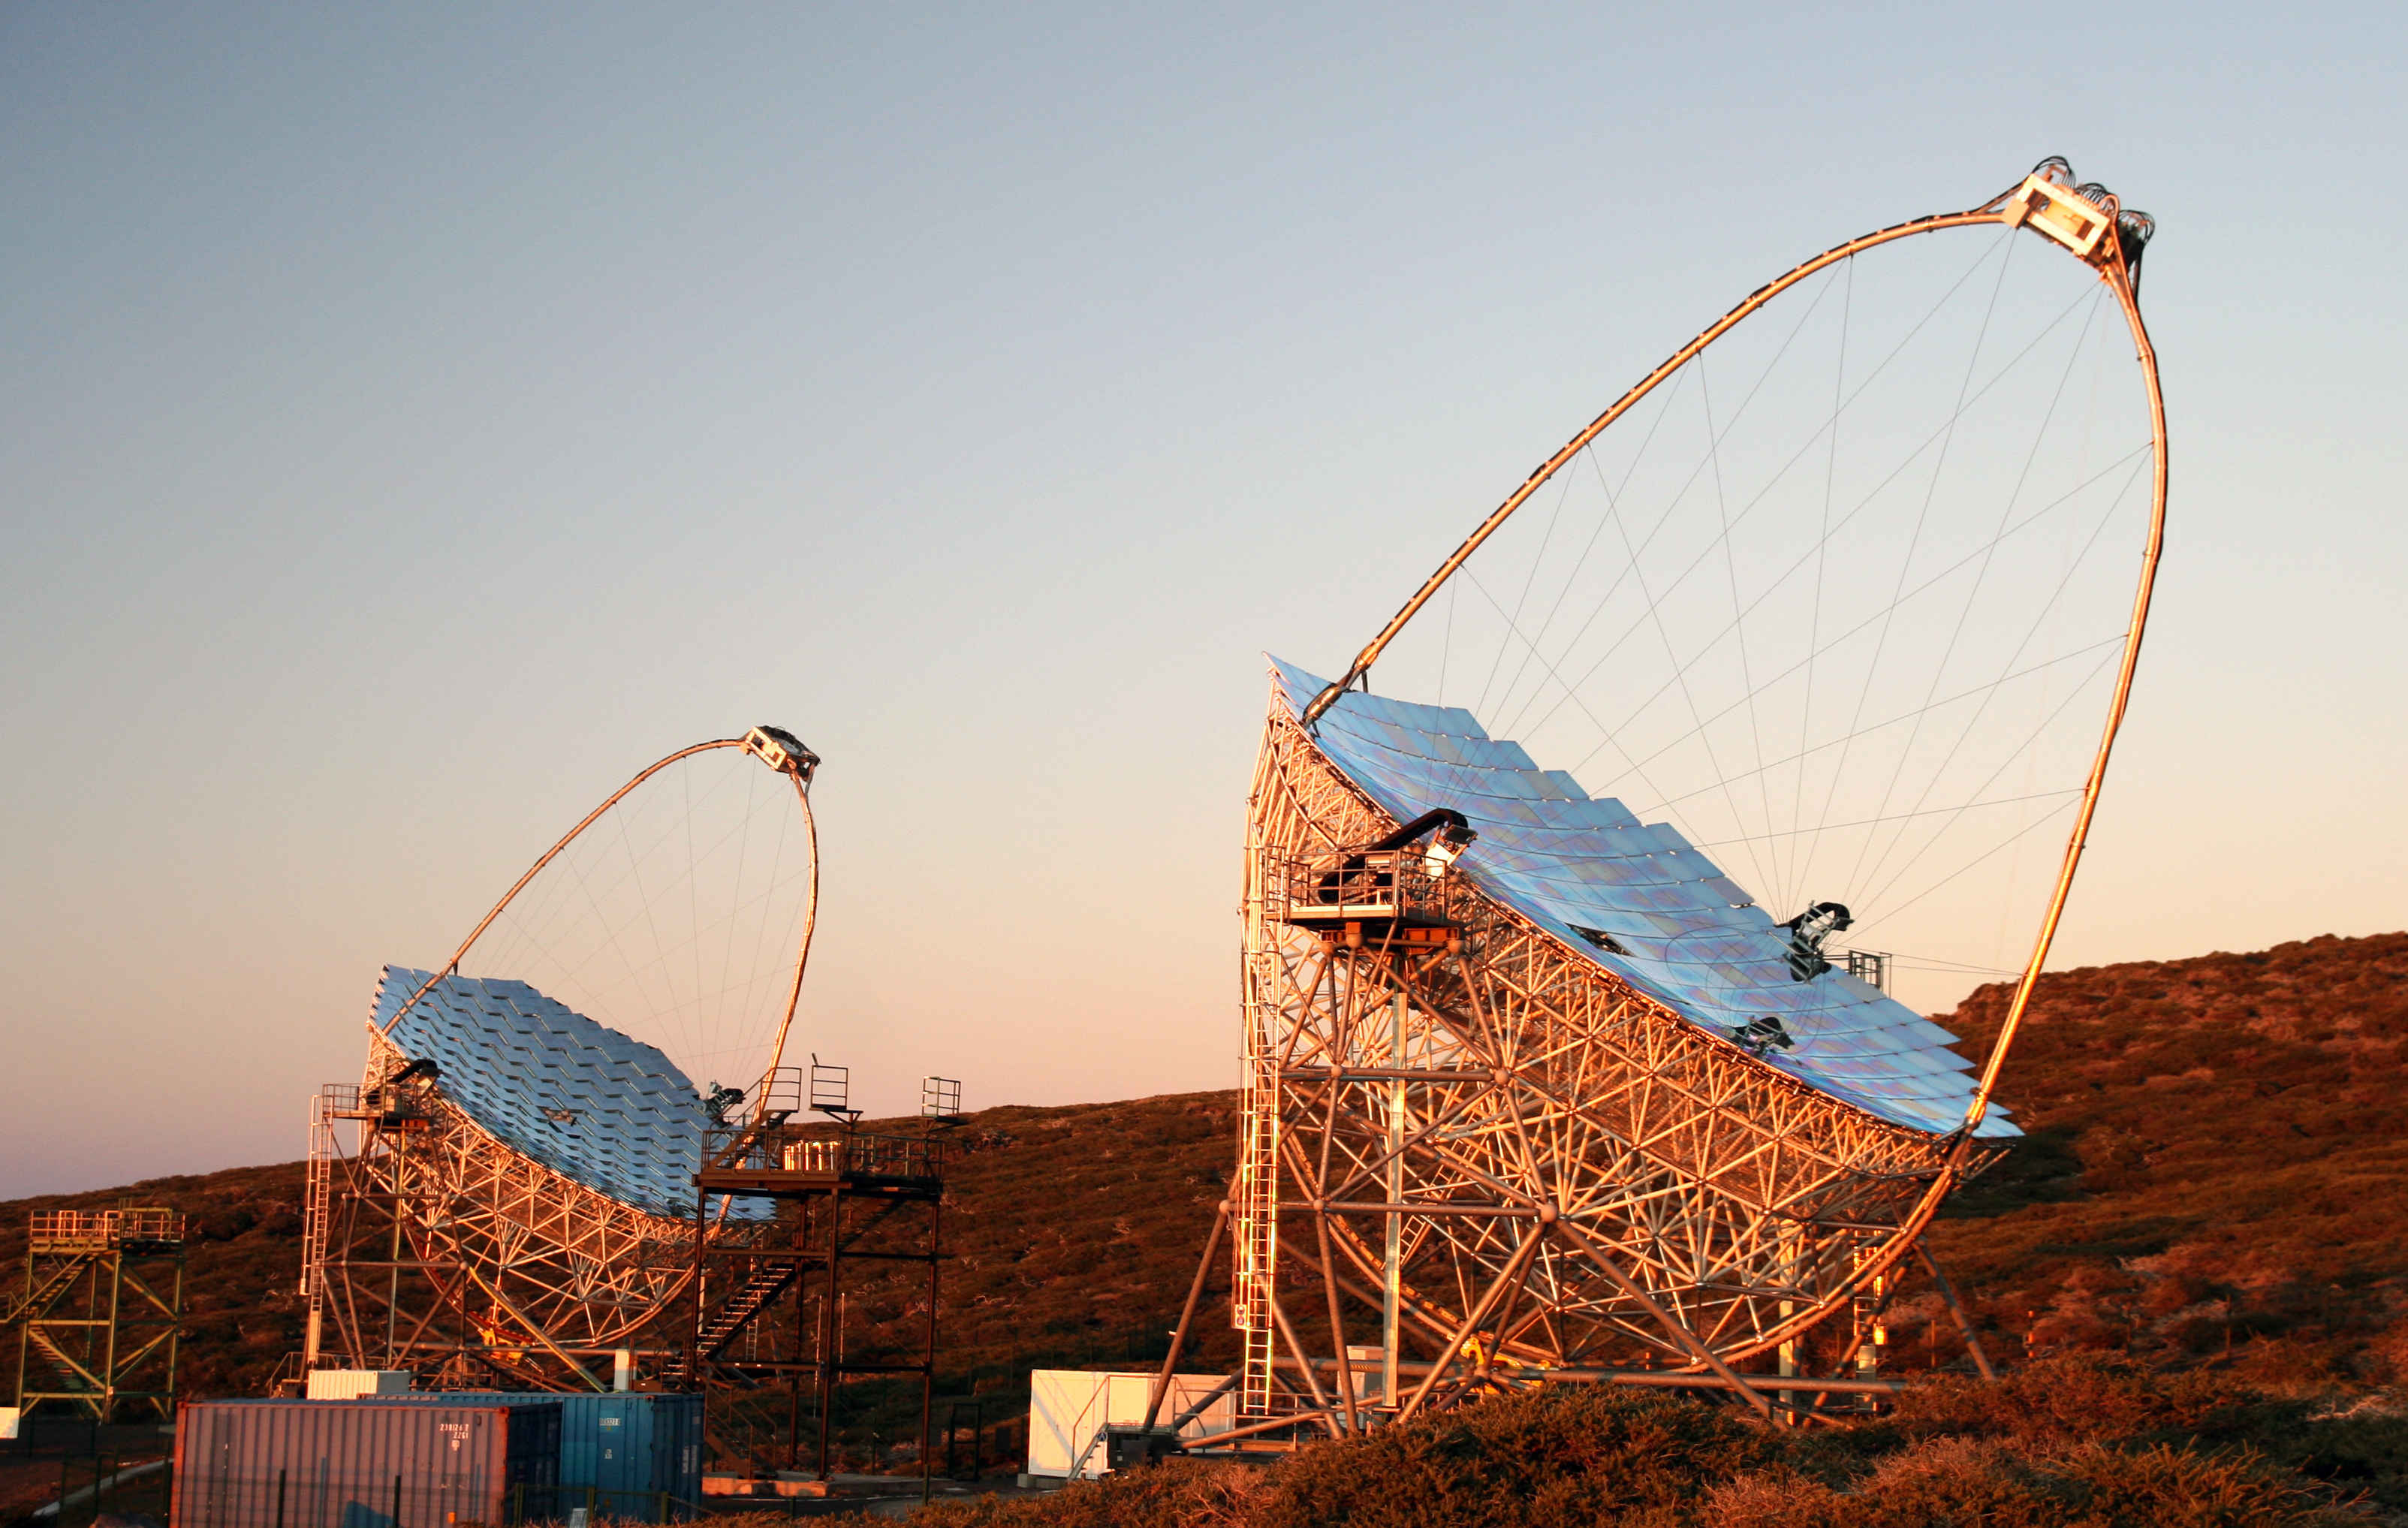
\includegraphics[width=\linewidth]{pictures/magic.JPG}
		\caption{MAGIC Teleskope in Observationsstellung.}%
		\label{fig:magic}
\end{wrapfigure}

Der Nachweis von hochenergetischer Gammastrahlung ist auf der Erde aufgrund der
Atmosphäre nur indirekt möglich.
Hochenergetische Primärteilchen, Photonen und Hadronen, erzeugen in der Atmosphäre
Teilchenschauer (siehe Abbildung~\ref{fig:schauer}), die aufgrund ihrer relativistischen Geschwindigkeiten Tscherenkowlicht abstrahlen.
\begin{wrapfigure}[13]{I}{0.45\textwidth}
		\includegraphics[width=\linewidth]{tikz/build/shower.pdf}
		\caption{Teilchen in einem Teilchenschauer mit einem Photon als
    Primärteilchen.}%
    \label{fig:schauer}
\end{wrapfigure}
MAGIC ist derzeit (16.11.2016) das größte Stereoteleskop
welches in einem Energiebereich von \SI{50}{\giga\electronvolt} bis
\SI{50}{\tera\electronvolt} sensitiv ist.
Es steht auf der Insel La Palma auf einer Höhe von \SI{2200}{\meter}.
Propagiert ein geladenes Teilchen mit einer Geschwindigkeit in einem
Medium, die höher als die Lichtgeschwindigkeit in diesem Medium ist,
so erzeugt dieses Tscherenkow-Photonen.
Die ultrarelativistischen Photonen, welche in die Erdatmosphäre eintreten,
wechselwirken mit den darin enthaltenen Teilchen beispielsweise über
Bremsstrahlung oder Paarerzeugung und produzieren somit weitere
relativistische Teilchen, welche wiederum Tscherenkowkegel erzeugen.
Dabei partitioniert das Primärteilchen die Energie solange, bis die Energie
nicht mehr ausreicht Sekundärteilchen zu produzieren.

Die dadurch erzeugten Lichtblitze können durch Tscherenkowteleskope gemessen
werden.
Die Spiegelfläche von \SI{17}{\meter} Durchmesser besteht aus \num{974} einzelnen
Spiegeln, die auf \num{1039} Photo Multiplier Tubes (PMTs) abbilden.
Das Teleskop besitzt ein Field of View von \SI{3.5}{\degree}.

Ziel ist es, mit den Teleskopen Gamma-Quellen wie AGNs, Supernovae und
Gasverteilungen, in denen viel Sternbildung stattfindet, zu observieren, um etwas
über die fundamentalen physikalischen Prozessen in der Quellregion zu erfahren.
Aufgrund der hohen Energien die bei stellaren Prozessen erzeugt werden, können
so Effekte auf Energieskalen beobachtet werden, welche nicht mit irdischen
Teilchenbeschleunigern erzeugt werden können.
Des Weiteren wird nach einen indirekten Nachweis nach dunkler Materie gesucht.
Fundamentales Problem ist, dass geladene Teilchen jegliche Richtungsinformation
in kosmologischen Magnetfeldern verlieren und somit keine Informationen zur
Quelle rekonstruiert werden kann.

\section*{Krebsnebel}%
\label{sec:krebsnebel}

In diesem Versuch wird der Krebsnebel untersucht.
Er ist ein Überrest einer Supernova-Explosion eines Sterns
mit 8~bis 12 Sonnenmassen aus dem Jahre 1054,
und befindet sich im Sternbild Stier.

\begin{wrapfigure}[16]{O}{0.35\textwidth}
		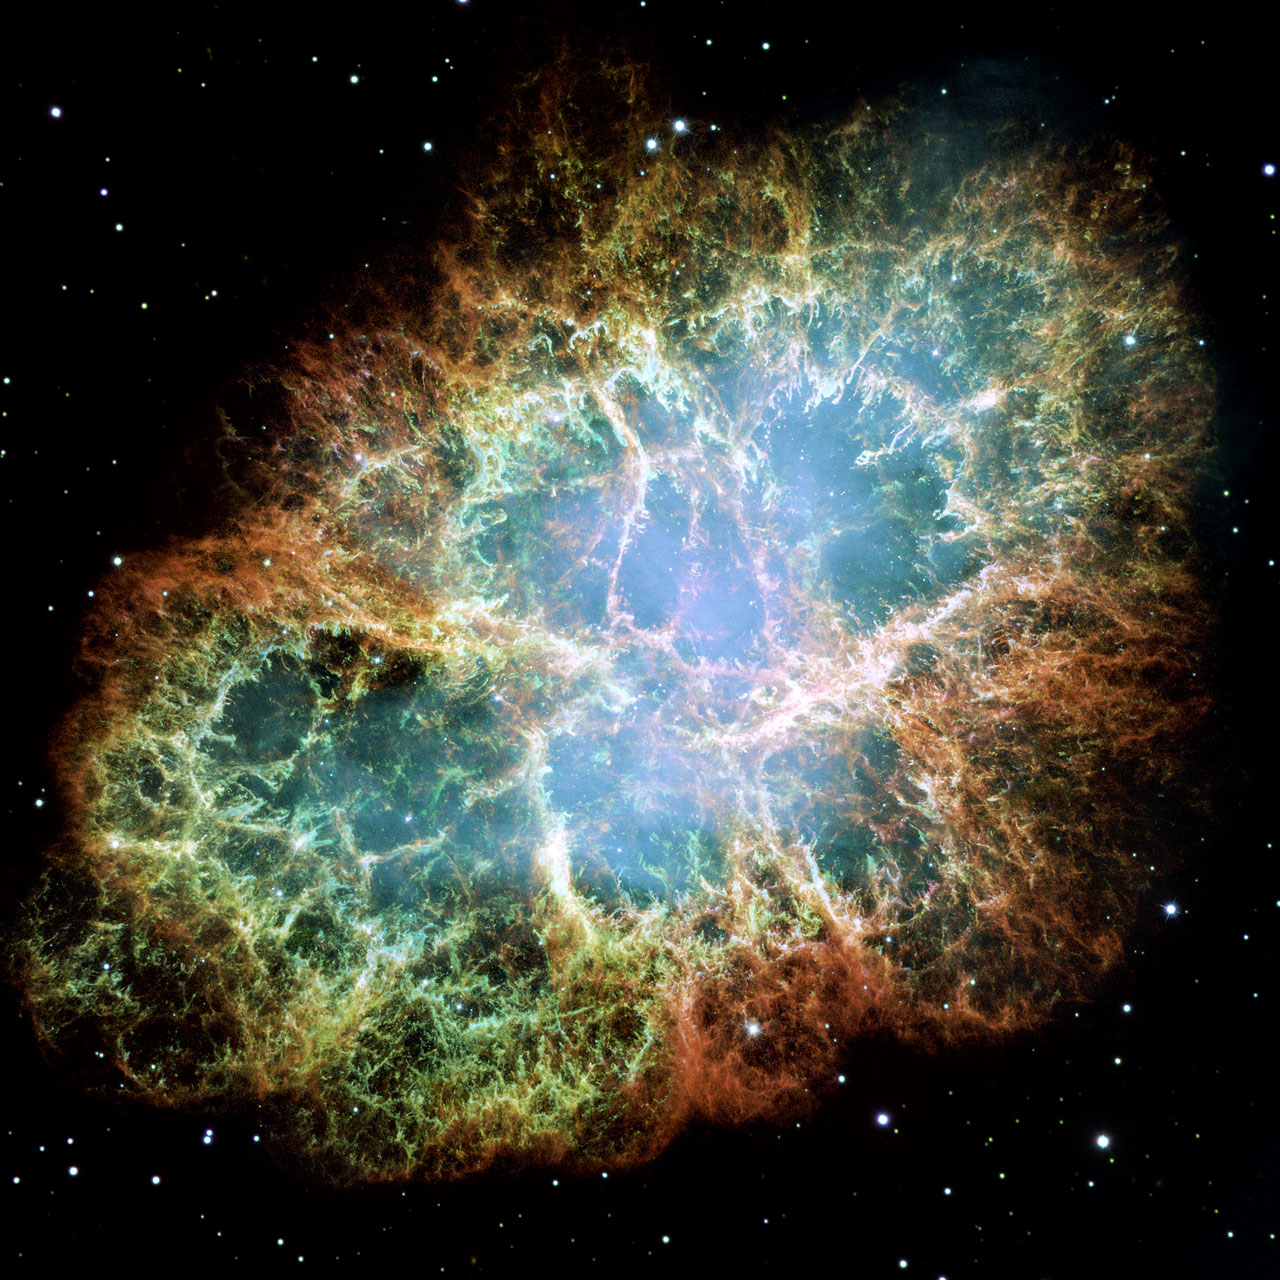
\includegraphics[width=\linewidth]{pictures/crab.jpg}
		\caption{Krebsnebel aufgenommen mit dem Hubble Teleskop.}%
		\label{fig:magic}
\end{wrapfigure}

Eine Supernova-Explosion ist das Ende eines massereichen Sterns,
bei dem die Leuchtkraft eines Sterns kurzzeitig auf das millonen- bis
milliardenfache der ursprünglichen Leuchtkraft anwächst,
ehe der Stern nach dem Verbrauch des
nuklearen Brennstoffs kollabiert und ein kompaktes Objekt
(Neutronenstern oder Schwarzes Loch) bildet.

Im Zentrum des Krebsnebel befindet sich ein Pulsar,
welcher die Quelle von starker elektromagnetischer Strahlung ist.
Pulsare sind schnell rotierende Neutronensterne,
welche sehr regelmäßige, kurze Pulse emittieren.
Typische Größen von Neutronensternen sind Durchmesser von einigen
\SI{10}{\kilo\meter}.
Die Materiereste, die bei einer Supernova-Explosion
vom zurückbleibenden Neutronenstern abgesprengt werden,
bilden eine überschallschnelle Schockwelle.
Diese heizt bei der Expansion das interstellare Medium auf Temperaturen von bis zu
\SI{e8}{\kelvin} auf.
Die propagierenden Schockwellen können durch Dichteschwankungen des stellaren
Mediums Sternbildung auslösen
und sind außerdem Lieferant für schwere Elemente, die in einem normalen
Fusionsprozess eines Sterns nicht gebildet werden können.

Aufgrund seiner Eigenschaften wird er als Standardkerze der Gamma-Astronomie betitelt,
da die Eigenschaften sehr gut bekannt sind
und der Gammafluss im hochenergetischen Bereich nicht variabel ist.
Durch seine Analyse kann die Performance von verschiedenen Teleskopen verglichen werden.

\subsection*{Detektion}%
\label{sub:wobbelmodus}

Da kosmische Quellen nicht isoliert von ihrer Umgebung betrachtet
werden können,
müssen zu jeder anvisierten Quellposition Umgebungsdaten aufgenommen werden.
Die
% wird zu jeder
Quellposition heißt \textit{On}.
% genau so lang Daten aufgenommen,
% wie
% und die
Positionen nahe der Quellposition,
in denen kein Gammafluss erwartet wird,
heißen \textit{Off}.

Die Teleskope triggern drei Arten von Events.
Neben den eigentlichen Luftschauern,
welche durch Protonen
oder Gammas verursacht werden,
erzeugen Myonen oder versehentliche Trigger weitere Events.
Myonen erzeugen ringförmige Ereignisse in der Kamera.
Versehentliche Trigger entstehen z.B.\ durch den Nachthimmelhintergrund
(\textit{Night Sky Background, NSB}) und elektronisches Rauschen.

In der Gamma Ray Astronomie werden die Teleskope in der Regel auf einen Punkt
ausgerichtet, an dem eine Quelle angenommen wird.
Die gemessenen Events, die das Teleskop triggert, können vom
kosmischen Hintergrund oder von einer echten Quelle, falls diese existiert, sein.

MAGIC nimmt Daten im Wobble-Modus auf.
Die erwartete Quellposition liegt dabei nicht im
Kameramittelpunkt,
sondern um
\SI{0.4}{\degree} um die Kameraachse
verschoben,
wobei die angenommene Quellposition um die Kameraachse rotiert wird.
In äquidistanten Abständen um die Kameraachse
werden Off-Positionen bestimmt (siehe Abbildung~\ref{fig:hillas}).
Dies hat den Vorteil, dass die Aufnahme von On und Off Daten zeitgleich möglich
ist und so die Messzeit maximiert wird.

% Anschließend wird der Abstand $\theta$ der rekonstruierten
% zu der On- und den Off-Positionen bestimmt.
% Die Bins von $\theta^2$ werden in den Off-Positionen
% anhand der On-Position (Anzahl Off-Positionen / Messzeiten) normiert.
% Im Anschluss wird der aus den Off-Positionen bestimmte Untergrund
% aus der Messung der On-Position subtrahiert, sodass Signal übrig bleibt
% (vgl. Abbildung~\ref{fig:thetacut}).

\clearpage
